\section{Link Budget}
\paragraph
\ Astrea constellation main satellite must be able to stablish three different telecommunications link: 
\begin{itemize}
	\item Space to Ground link for payload and TT\&C data.
	\item Space to Space link between Astrea satellites.
	\item Space to Space link between client and Astrea satellites.
\end{itemize} 
\subsection{Communications Basics}
\paragraph
\

When evaluating a wireless link, the three most important questions to be answered are: \cite{Note1998}\\
\begin{enumerate}
	\item \underline{How much radio frequency (RF) power is available?}
	Up to 2W for S band or up to 12W for Xband.
	\item \underline{How much bandwidth is available?}\\
	Available 400MHz with 28 channels of 14MHz or 228 channels of 1.75MHz for inter-satellite communication at S band. For X band, there's more than 4GHz available \cite{SecretariadeEstadodetelecomunicacionesyparalasociedaddelainformacion.2015}. In fact is limited by the TR-600 transceiver at 56MHz for S band and to 100MHz by SWIFT - XTS at X band.
	\item \underline{What is the required reliability (as defined by Bit Error Rate, or BER)?}\\
	Required reliability for space systems$E_b/N_o \geq 10$, so $BER=5.5x10^{-6}$ for a MSK, PSK (worst case) modulation as shown in Fig.\ref{BEvsSNR}.
\end{enumerate}
The upper limit in terms of data rate is given by Shannon's Channel Capacity Theorem:
\begin{equation}
	C=Blog_2(1+S/N)
	\label{channelCapacity}
\end{equation}
where:
\begin{align*}
	C&= \text{channel capacity (bits/s)}\\
	B&= \text{channel bandwidth (Hz)}\\
	S&= \text{signal strength (watts)}\\
	N&= \text{noise power (watts)}
\end{align*}

\paragraph{} With all data known, the minimum required sensitivity of a receiver using the Eq. \ref{channelCapacity} will be stated in the Link Budget calculation.

\paragraph{Transmission Losses}
\ In any satellite transmission, there are always losses from various sources. Some of
those losses may be constant, others are dependent of statistical data and others vary
with the weather conditions, especially with rain.

\begin{figure}[h]
	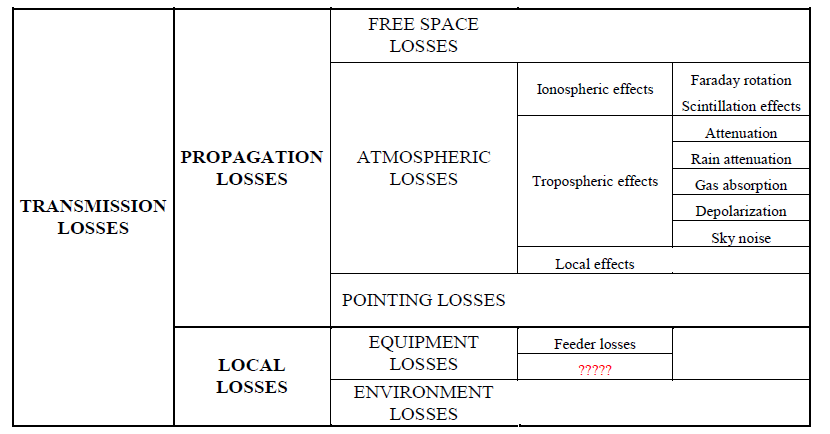
\includegraphics[scale=0.8]{./sections/SatelliteDept/sections/images/principal_losses}
	\centering
	\caption{Principal losses in the received signal \cite{Jorge2012}}
	\label{principal_losses}
\end{figure}

\subsection{Propagation losses}
\subsubsubsection{Free Space Losses}
\paragraph{Range and Path Loss}
\
Another key consideration is the issue of range. As radio waves propagate in free space, power falls off as the square of range. For a doubling of range, power reaching a receiver antenna is reduced by a factor of four. This effect is due to the spreading of the radio waves as they propagate, and can be calculated by \cite{Note1998}:
\begin{equation}
L=20log_{10}(4\pi D/\lambda)
\label{FSP}
\end{equation}
where:
\begin{align*}
	D&= \text{the distance between receiver and transmitter}\\
	\lambda&= \text{free space wavelength = c/f}\\
	c&= \text{speed of light}(3\mathrm{x}10^8m/s)\\
	f&= \text{frequency (Hz)}
\end{align*}
\clearpage
\subsubsubsection{Atmospheric Losses}
\paragraph \ This kind of losses derives from the absorption of energy by atmospheric gases. They can assume two different types:
\begin{itemize}
	\item Atmospheric attenuation.
	\item Atmospheric absorption.
\end{itemize}

The major distinguishing factor between them is their origin. Attenuation is weatherrelated, while absorption comes in clear-sky conditions.
Likewise, these losses can be due to ionospheric, tropospheric and other local effects. \cite{Jorge2012}
\paragraph{Ionospheric Effects}
\ All radio waves transmitted by satellites to the Earth or vice versa must pass through the
ionosphere, the highest layer of the atmosphere, which contains ionized particles,
especially due to the action of sun’s radiation. Free electrons are distributed in layers
and clouds of electrons may be formed, originating what is known as travelling
ionospheric disturbances, what provoke signal fluctuations that are only treated as
statistical data. The effects are:
\begin{itemize}
	\item \textbf{Polarization rotation}: When a radio wave passes through the ionosphere, it contacts the layers of ionized 	electrons that move according to the Earth’s magnetic field. The direction these 	electrons move will no longer be parallel to the electric field of the wave and therefore	the polarization is shifted, in what is called Faraday rotation ($\theta_F$). ;
	\item \textbf{Scintillation effects}: Differences in the atmospheric refractive index may cause scattering and multipath 	effect, due to the different directions rays may take through the atmosphere. They are detected as variations in amplitude, phase, polarization and angle of arrival of	the radio waves.	It is often recommended the introduction of a fade margin so atmospheric scintillation
	can be a tolerated phenomenon.; 
	\item Absorption
	\item Variation in the direction of arrival
	\item Propagation delay
	\item Dispersion
	\item Frequency change
\end{itemize}
These effects decrease usually with the increase of the square of the frequency and most serious ones in satellite communications are the polarization rotation and the
scintillation effects, and those are the ones that will be treated in this dissertation. \cite{Jorge2012}
\paragraph{Tropospheric Effects \cite{Jorge2012}}
\ Troposphere is composed by a miscellany of molecules of different compounds, such as hail, raindrops or other atmospheric gases. Radio waves that pass by troposphere will suffer their effects and will be scattered, depolarized, absorbed and therefore attenuated.\\
\underline{Attenuation}: As radio waves cross troposphere, radio frequency energy will be converted into thermal energy and that attenuates signal.\\
\underline{Rain attenuation}: Ground stations had been chosen in order that the attenuation caused by rainfall will be very punctual. Also, the fact that there are three ground stations makes really difficult that a satellite can not communicate to the ground in all the orbit period.\\
\underline{Gas absorption}: Under normal conditions, only oxygen and water vapour have a significant contribution
in absorption. Other atmospheric gases only become a problem in very dry air
conditions above 70 GHz.
Thereby, losses caused by atmospheric absorption vary with frequency and the
collection of data already received allows the elaboration of the graphic that follows:
\begin{figure}[h]
	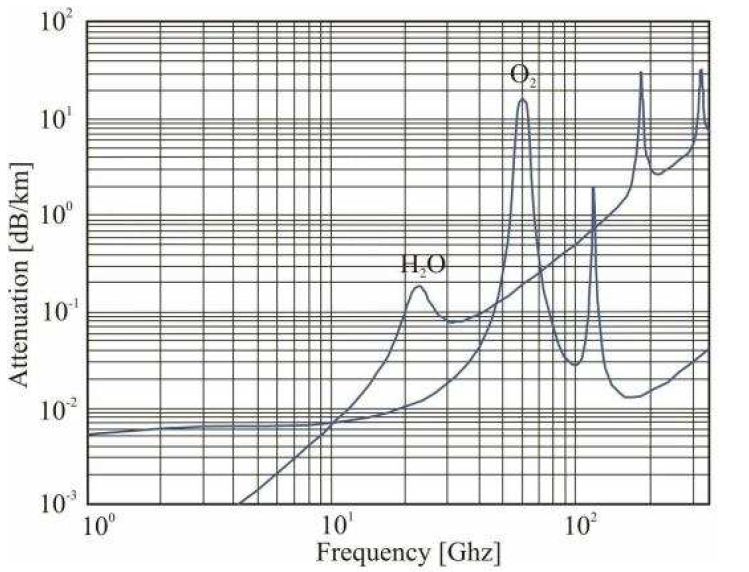
\includegraphics[scale=0.7]{./sections/SatelliteDept/sections/images/specificAttenuation}
	\centering
	\caption{Specific attenuation for different frequencies \cite{Jorge2012}}
	\label{specificAtenuattion}
\end{figure}
\\

Once these values depend on atmosphere thickness, it becomes necessary to perform all calculations taking into account troposphere’s thickest layer ($T_{trop}$), which has 20 km.\\
It is also mandatory to refer that this graph represents the absorption for a satellite in the zenith, in other words, for an elevation angle of 90º ($\theta$ = 90º). For lower angles, the atmospheric absorption ($L_{abs}$) is given by \cite{Jorge2012}:
\begin{equation}
	L_{abs}(dB)=L_{abs|90º} (dB/km)\ cosec(\theta)\ T_{trop}(km)
	\label{Labs}
\end{equation}
\paragraph{} For AstreaSAT, $5\mathrm{x}10^{-3}dB/km$ attenuation factor is considered for S band due to the $O_2$ specific attenuation. On the other hand, $4\mathrm{x}10^{-3}dB/km$ attenuation factor is considered for X band due to the $H_2O$ and to the $O_2$ specific attenuations. An study of the critical elevation angle will lately be performed. 
\paragraph{} For AstreaSAT ground station, communication starts at an elevation angle of $\theta=10^o$ (worst case scenario). Consequently, $cosesc(\theta)$ will go from 5.76 to 1 (best reception case). In that case, we assume:
\begin{align*}
	L_{abs}=2\cdot4\mathrm{x}10^{-3}\cdot5.76\cdot20 =\textbf{0.92dB} \quad \text{X band}\\
	L_{abs}=5\mathrm{x}10^{-3}\cdot5.76\cdot20 =\textbf{0.58dB} \quad \text{S band}
\end{align*}

\underline{Polarization}: Satellite communications use linear and circular polarization, but undesirable effects may transform it into an elliptical polarization. Depolarization may occur when an orthogonal component is created due to the passing of the signal through the ionosphere. There are two ways to measure its effect, cross polarization discrimination (XPD) and polarization isolation (I)\cite{Jorge2012}. To overcome this attenuation problems a circular polarization is the best option. AstreaSAT patch antennas will mitigate this problem, therefore this loses are considered negligible.\\

\underline{Sky noise}: Sky noise is a combination of galactic and atmospheric effects, according as both these factors influence the quality of the signal in the reception. Galactic effects decrease with the increase of frequency. They are due to the addition of the cosmic background radiation and the noise temperature of radio stars, galaxies and nebulae. This value is quite low and a good approximation is \textbf{3 K}.
\begin{figure}[h]
	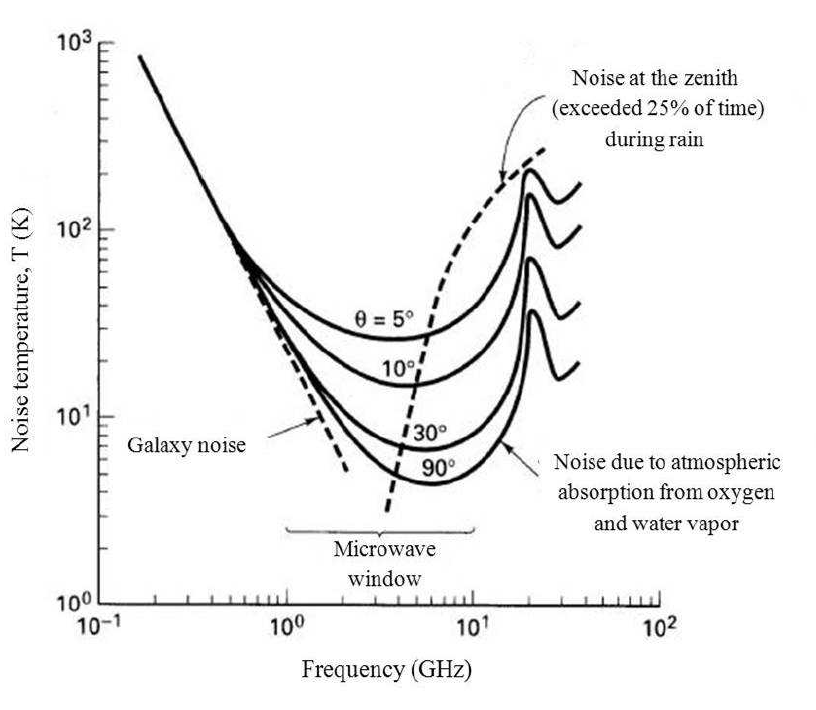
\includegraphics[scale=0.5]{./sections/SatelliteDept/sections/images/NoiseTemperature}
	\centering
	\caption{Galaxy noise influence in noise temperature \cite{Jorge2012}}
	\label{NoiseTemperature}
\end{figure}
\begin{figure}[h]
	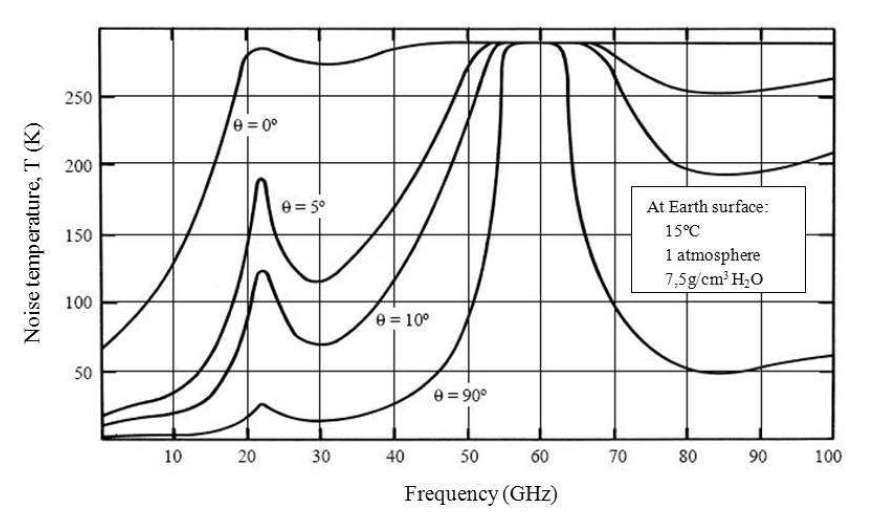
\includegraphics[scale=0.55]{./sections/SatelliteDept/sections/images/NoiseTemperature2}
	\centering
	\caption{Noise temperature variation with frequency \cite{Jorge2012}}
	\label{NoiseTemperature2}
\end{figure}
\paragraph{AstreaSAT noise temperature} A good approximation based on Fig.\ref{NoiseTemperature} is that Galaxy noise is 3K for S band and almost 1K for X band. Furthermore, for the previous worst case scenario stated before $\theta=10$, noise temperature due to atmospheric absorption is 19K for both bands (S and X).
\clearpage
\paragraph{Local Effects}
These effects refer to the proximity of the local ground stations, possible sources that may interfere with the received signal and buildings that may block the signal. If the ground station is on a free external interferences zone, for satellite communications this factor may be negligible.
\subsubsubsection{Pointing Losses}
\paragraph
\
Ideal reception implies that the value for misalignment losses would be 0 dB which
means maximum gain at the ground station is achieved when both the transmitter and
the receiver antennas are 100\% aligned. Realistically it is virtually impossible to
achieve a perfect alignment between the antennas of the ground station and the satellite,
especially in the case of CubeSats, due to their fast movement of nearly $8000\ ms^{-1}$.
\paragraph{}
Antenna misalignment losses ($L_{aml}$) are calculated using statistical data, so these values
are an approximation based on real data observed in several GS. Ergo, these values are
not calculated, but estimated.\cite{Jorge2012}
 \paragraph{} Based on a estimation from \cite{Macdonald2014} a $L_{aml}=1dB$ is a good approximation.
\subsubsubsection{Multipath and Fade Margin}
\paragraph
\
Multipath occurs when waves emitted by the transmitter
travel along a different path and interfere destructively with
waves travelling on a direct line-of-sight path. This is
sometimes referred to as signal fading. This phenomenon
occurs because waves travelling along different paths may
be completely out of phase when they reach the antenna,
thereby cancelling each other.\\

The amount of extra RF power radiated to overcome this
phenomenon is referred to as fade margin. The exact
amount of fade margin required depends on the desired
reliability of the link, but a good rule-of-thumb is 20dB to
30dB.


\subsection{Local Losses}
\subsubsubsection{Equipament Losses}
\paragraph{}The receiving and emitting equipments also introduces some losses to the signal.\\
\underline{Feeder Losses}: Feeder losses occur in the several components between the receiving antenna and the
receiver device, such as filters, couplers and waveguides. These losses are similar to the
ones which occur also in the emission, between the emitting antenna and the output of
the high power amplifier (HPA).\cite{Jorge2012}

\subsubsubsection{Environment Losses}
\paragraph{}
This item is related to the specific region of the globe where the ground station is placed
(equatorial, tropical, polar…). Depending on its latitude, each region has its own
characteristics (e.g. temperature, moisture, thickness of atmospheric ice layer…), which
may provoke variation in signal reception. \cite{Jorge2012}
\paragraph{} Communications department, had chosen the best locations over the globe, with stable good weather conditions to neglect this fact.
\subsection{Modulation Technique}
\paragraph
\ Modulation technique is a key consideration. This is the
method by which the analogue or digital information is
converted to signals at RF frequencies suitable for
transmission. Selection of modulation method determines
system bandwidth, power efficiency, sensitivity, and
complexity. Most of us are familiar with Amplitude
Modulation (AM) and Frequency Modulation (FM) because
of their widespread use in commercial radio. Phase
Modulation is another important technique. It is used in
applications such as Global Position System (GPS)
receivers and some cellular telephone networks. \cite{Note1998}\\

For the purposes of link budget analysis, the most important
aspect of a given modulation technique is the Signal-to-
Noise Ratio (SNR) necessary for a receiver to achieve a
specified level of reliability in terms of BER.\\

\begin{figure}[h]
	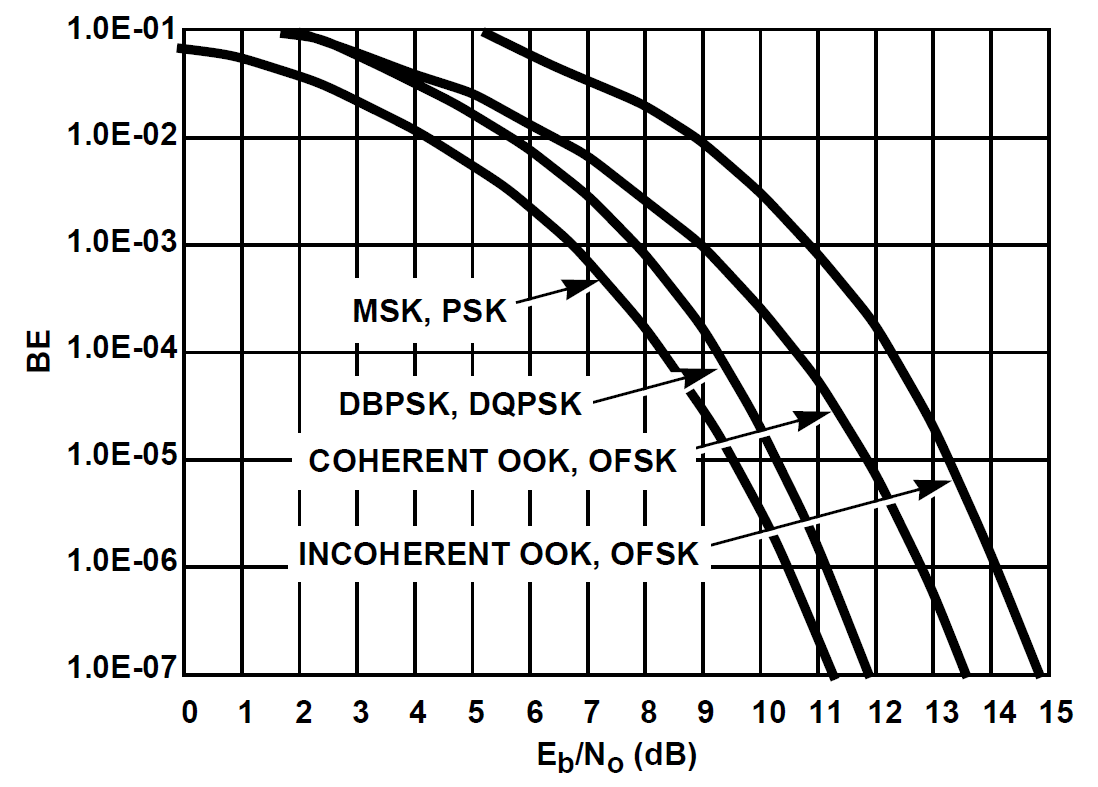
\includegraphics[scale=0.3]{./sections/SatelliteDept/sections/images/BEvsSNR}
	\centering
	\caption{Probability of bit error for common modulation methods \cite{Note1998}}
	\label{BEvsSNR}
\end{figure}
\pagebreak
A graph of $E_b/N_o$
vs BER is shown in Figure \ref{BEvsSNR}. $E_b/N_o$ is a measure of the
required energy per bit relative to the noise power. Note that
$E_b/N_o$ is independent of the system data rate. In order to
convert from $E_b/N_o$ to $SNR$, the data rate and system
bandwidth must be taken into account as shown below:
\begin{equation}
SNR=(E_b/N_o)(R/B_T)
\label{SNReq}
\end{equation}
where:
\begin{align*}
	E_b&= \text{Energy required per bit of information}\\
	N_o&= \text{thermal noise in 1Hz of bandwidth}\\
	R&= \text{system data rate}\\
	B_T&= \text{system bandwidth}
\end{align*}

\paragraph{} AstreaSAT is equipped with Software Defined Radios, it has the ability to change the modulation methods when its flying, for calculus MSK and PSK modulations will be considered, because of their more restrictive conditions.

\subsection{System Noise}
The system noise temperature ($T_S$) is the sum of the antenna noise temperature ($T_A$) and
the composite temperature of other components ($T_{comp}$), according to:    \cite{Jorge2012}
\begin{equation}
T_S=T_A+T_{comp}
\end{equation}

$T_A$ may be known if the total attenuation due to rain and gas absorption (A), the
temperature of the rain medium ($T_m$) and the temperature of the cold sky ($T_C$) are also
known. Then, the following expression may be applied:
\begin{equation}
	T_A=T_m\ (1-10^{-A/10})+T_C\ 10^{-A/10}
\end{equation}

Usually, for clouds it is considered $T_m=280K$ and for the rain $T_m=260K$. The sky noise tends to be $T_C=10K$. Taking into account the values from Fig.\ref{NoiseTemperature} and Fig.\ref{specificAtenuattion} the following estimation can be made:
\begin{align*}
	T_A=280\cdot (1-10^{-(5\mathrm{x}10^{-3})/10})+22\cdot 10^{-(5\mathrm{x}10^{-3})/10}&=\textbf{22.29K} \quad \text{S band} \\
	T_A=280\cdot (1-10^{-2\cdot(4\mathrm{x}10^{-3})/10})+20\cdot 10^{-2\cdot(4\mathrm{x}10^{-3})/10}&=\textbf{20.48K} \quad \text{X band} 
\end{align*}

\paragraph{} According to \cite{Jorge2012} a good components temperature approximation for a typical ground station is $T_{comp}=65.5K$.

\paragraph{} AstreaSAT system temperature will be considered as $T_S=22.29+65.5=\textbf{87.79K}$ for S band and $T_S=20.48+65.5=\textbf{85.98K}$ for X band. Since both frequencies are part of the microwave spectrum, we see that system temperatures are pretty much the same.

\paragraph{Channel Noise}\
All objects which have heat emit RF energy in the form of random (Gaussian) noise. The amount of radiation emitted can be calculated by \cite{Note1998}:
\begin{equation}
N=kTB
\label{noise}
\end{equation}
where:
\begin{align*}
	N&= \text{noise power (watts)}\\
	k&= \text{Boltzman's constant}(1.38\mathrm{x}10^{-23}J/K)\\
	T&= \text{system temperature, usually assumed to be 290K}\\
	B&= \text{channel bandwidth (Hz)}
\end{align*}

This is the lowest possible noise level for a system with a given physical temperature. For most applications, temperature is typically assumed to be room temperature (290K). Equations \ref{channelCapacity} and \ref{noise} demonstrate that RF power and bandwidth can be traded off to achieve a given performance level (as defined by BER). \cite{Note1998}

\subsection{Link Budget Calculation}
\paragraph{Methodology} \ From the expected requirements fixed on the Project Charter, general radio systems parameters will computed, in order to have a reference to look for the best communications system on board the Astrea satellites. As background, general losses parameters had been calculated on previous sections. 

\paragraph{} The most important concern on AstreaSAT link Budget is how far every satellite can emit on the desired frequencies. This is a key factor to know the utility of the modules selected. At least, Project Charter communication requirements must be accomplish.
 
$EIRP=P_T-L_T-G_T$\\
FRIIS EQUATION + GRAPH RANGE\\
SENSITIVITY CALCULUS A PARTIR DE LA DE CAPACITAT + NOISE ADJUDICANT BANDWITH
